\chapter{रसायन विज्ञान में कृत्रिम बुद्धिमत्ता}
\label{ch:chemistry}

\lakshyaheading
\begin{itemize}[leftmargin=1.4em]
  \item अणु (molecule) एवं अभिक्रिया (reaction) को \emph{data} के रूप में देखना।
  \item आवर्त सारणी (periodic table) के गुणों में pattern एवं प्रवृत्ति (trend) पहचानना।
  \item \term{वर्गीकरण}{classification} एवं \term{पूर्वानुमान}{prediction} द्वारा
        पदार्थों के गुण आँकना।
  \item दवा-खोज (drug discovery) एवं नई सामग्री (materials) में AI की भूमिका।
  \item मुफ़्त उपकरणों से अणु एवं data पर स्वयं प्रयोग करना।
\end{itemize}

\section{अणु भी एक data हैं}

प्रत्येक अणु को उसके परमाणुओं (atoms) एवं उनके बीच के बंधों (bonds) की एक संरचना
(structure) के रूप में लिखा जा सकता है। यदि इस संरचना को संख्याओं में बदल दिया जाए, तो
कंप्यूटर लाखों अणुओं की आपस में तुलना कर सकता है और बता सकता है कि कौन-सा अणु किसी विशेष
\term{गुण}{property} वाला हो सकता है।

एक प्रचलित तरीका है \eterm{SMILES notation}, जिसमें अणु को एक छोटी
पंक्ति (string) के रूप में लिखते हैं। उदाहरण के लिए, जल (H\textsubscript{2}O) को \texttt{O},
तथा एथेनॉल को \texttt{CCO} लिखा जाता है। AI ऐसे संकेतों को पढ़कर अणु को ``समझ'' लेती है।
किसी अणु की त्रि-आयामी (3D) संरचना भी data ही है, जैसा चित्र~\ref{fig:caffeine} में
कैफ़ीन (caffeine) अणु के लिए दिखाया गया है।

\begin{figure}[h]
\centering
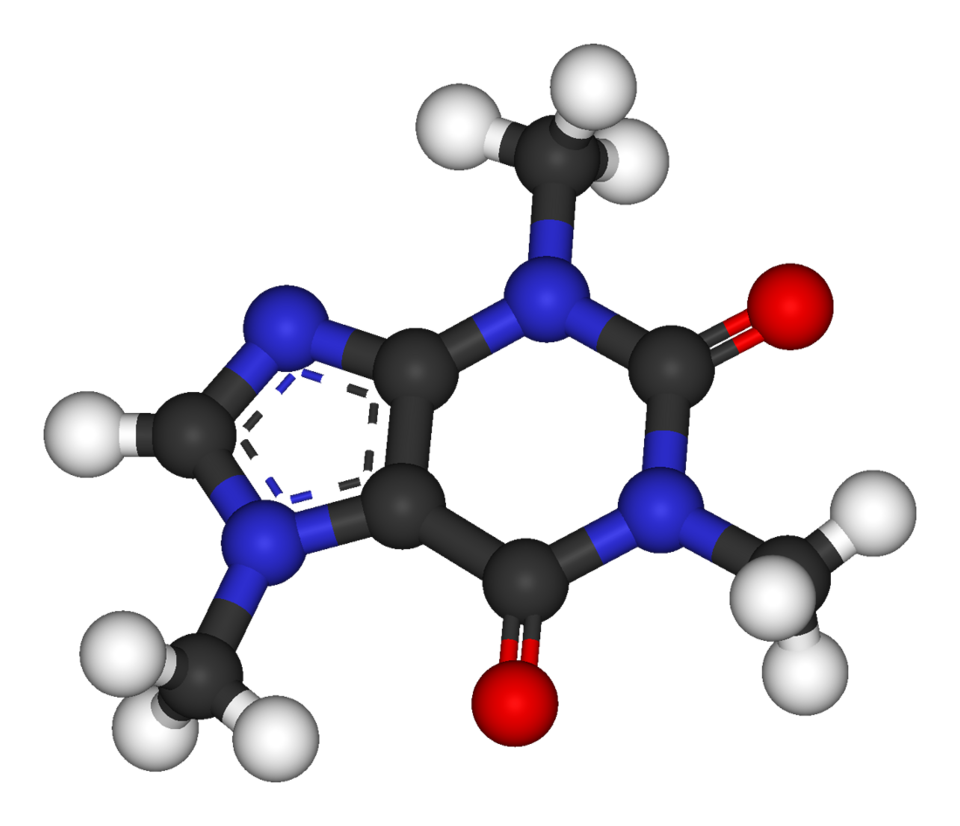
\includegraphics[width=0.45\linewidth]{images/caffeine.png}
\caption[कैफ़ीन अणु का त्रि-आयामी model]{कैफ़ीन अणु का त्रि-आयामी (ball-and-stick) model --
परमाणु एवं बंध ही वह ``data'' हैं जिन्हें AI पढ़ती है।\imgsrc{Wikimedia Commons (Public Domain)}}
\label{fig:caffeine}
\end{figure}

\begin{jante}
दुनिया में सैद्धांतिक रूप से सम्भव \emph{औषधि-सदृश} (drug-like) छोटे कार्बनिक अणुओं
की संख्या $10^{60}$ से भी अधिक आँकी गई है - इतने अणुओं को मनुष्य कभी हाथ से नहीं जाँच सकता, पर
AI उन्हें छाँट (screen) सकती है।
\end{jante}

\section{pattern: आवर्त सारणी की भाषा}

रसायन विज्ञान में पैटर्न-पहचान का सबसे सुंदर उदाहरण स्वयं \term{आवर्त सारणी}{Periodic
Table} है। मेंडेलीफ़ (Mendeleev) ने तत्वों के गुणों में प्रवृत्ति देखकर न केवल उन्हें
क्रम में रखा, बल्कि कुछ \emph{अनदेखे तत्वों} के गुणों का \emph{पूर्वानुमान} भी कर दिया -
जो बाद में सही निकले। यही ``data से पूर्वानुमान'' का विचार आज ML करता है।

\begin{table}[h]
\centering
\begin{tabular}{@{}p{4.6cm} p{8.4cm}@{}}
\toprule
\rowcolor{cvBlue}\hdc{प्रवृत्ति (trend)} & \hdc{आवर्त में (बाएँ से दाएँ) क्या होता है} \\
\midrule
परमाणु त्रिज्या (atomic radius) & घटती है \\
आयनन ऊर्जा (ionisation energy)  & बढ़ती है \\
विद्युत्‌ऋणात्मकता (electronegativity) & बढ़ती है \\
\bottomrule
\end{tabular}
\caption{आवर्त सारणी में दिखने वाली नियमित प्रवृत्तियाँ - pattern का आधार}
\end{table}

\begin{sochiye}
मेंडेलीफ़ ने ``eka-silicon'' (बाद में Germanium) के गुणों का पूर्वानुमान बिना उस तत्व
को देखे किया। उन्होंने किस आधार पर यह किया, और यह आज के Machine Learning के
``prediction'' से किस प्रकार मिलता-जुलता है? चर्चा कीजिए।
\end{sochiye}

\section{वर्गीकरण एवं पूर्वानुमान (Classification \& Prediction)}

रसायन में AI के दो सबसे सामान्य कार्य हैं:
\begin{itemize}[leftmargin=1.4em]
  \item \textbf{वर्गीकरण (classification):} किसी पदार्थ को श्रेणियों में बाँटना -
        जैसे ``अम्ल या क्षार'', ``विलेय या अविलेय'', ``विषैला या सुरक्षित''।
  \item \textbf{पूर्वानुमान (regression/prediction):} किसी सतत गुण का मान आँकना -
        जैसे क्वथनांक (boiling point), घुलनशीलता (solubility) या अभिक्रिया की दर
        (rate)।
\end{itemize}

इन दोनों के लिए मशीन को पहले बहुत-से ज्ञात उदाहरण (training data) दिए जाते हैं - जैसे
हज़ारों अणु और उनके मापे गए क्वथनांक। मशीन इनसे सम्बन्ध सीखकर किसी \emph{नए} अणु का
क्वथनांक बता देती है।

\begin{gatividhi}[आवर्त सारणी में प्रवृत्ति का ``regression'']
\textbf{लक्ष्य:} data में रुझान पहचानकर एक अनदेखे मान का पूर्वानुमान करना।\\[4pt]
\textbf{सामग्री:} ग्राफ़ पेपर, आवर्त सारणी (डेटा-पुस्तिका)।\\[4pt]
\textbf{चरण:}
\begin{enumerate}[leftmargin=1.6em]
  \item आवर्त-2 के तत्वों (Li, Be, B, C, N, O, F) का परमाणु क्रमांक एवं परमाणु
        त्रिज्या एक तालिका में लिखें।
  \item परमाणु क्रमांक (x) बनाम त्रिज्या (y) का ग्राफ़ बनाएँ।
  \item बिना मान देखे, किसी एक तत्व को छिपाकर उसकी त्रिज्या का पूर्वानुमान करें।
  \item वास्तविक मान से तुलना करें - आपकी त्रुटि कितनी रही?
\end{enumerate}
\textbf{अवलोकन:} आपने वही किया जो एक ML ``regression'' model करता है - ज्ञात बिंदुओं से
अनदेखे मान का अनुमान।
\end{gatividhi}

\section{दवा-खोज में AI (Drug Discovery)}

एक नई दवा बनाने में सामान्यतः 10–15 वर्ष एवं हज़ारों करोड़ रुपये लग जाते हैं, क्योंकि
लाखों अणुओं में से सही अणु खोजना पड़ता है। AI इस प्रक्रिया को इस प्रकार तेज़ करती है:

\begin{enumerate}[leftmargin=1.6em]
  \item \term{आभासी छँटाई}{Virtual Screening} - कंप्यूटर पर ही लाखों अणुओं को
        जाँचकर सम्भावित दवाओं की छोटी सूची बनाना।
  \item \term{गुण-पूर्वानुमान}{Property Prediction} - विषाक्तता (toxicity) एवं
        घुलनशीलता पहले से आँकना, ताकि असफल अणु जल्दी हट जाएँ।
  \item \term{अणु-अभिकल्प}{Molecule Design} - वांछित गुण वाले नए अणु ``सुझाना''।
\end{enumerate}

\begin{figure}[h]
\centering
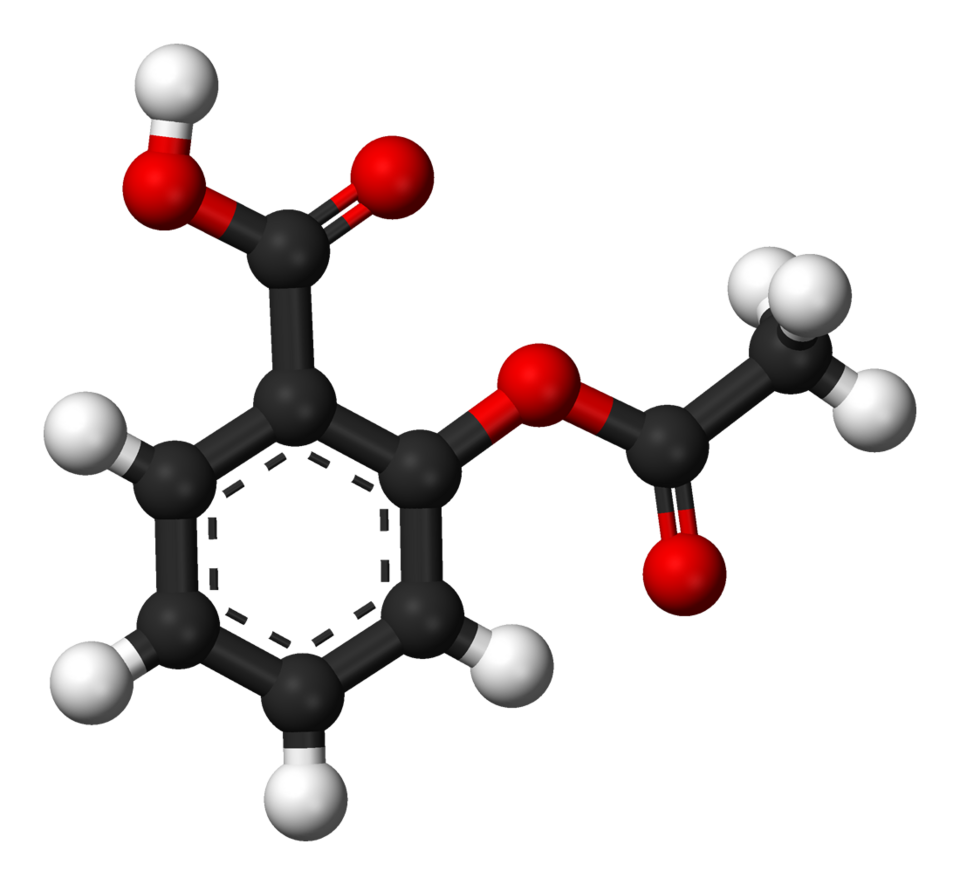
\includegraphics[width=0.45\linewidth]{images/aspirin.png}
\caption[एस्पिरिन अणु का 3D model]{एस्पिरिन (aspirin) अणु का 3D model -- AI ऐसे हज़ारों
दवा-अणुओं की संरचना एवं गुणों की तुलना कर सम्भावित औषधियाँ छाँटती है।\imgsrc{Wikimedia Commons (Public Domain)}}
\label{fig:aspirin}
\end{figure}

\begin{jante}
सन् 2020 में MIT के शोधकर्ताओं ने एक AI model से \emph{Halicin} नामक नया एंटीबायोटिक
खोजा। यह दवा परम्परागत एंटीबायोटिक से संरचना में बिल्कुल भिन्न थी, और कई दवा-प्रतिरोधी
(drug-resistant) बैक्टीरिया पर भी कारगर निकली।
\end{jante}

\section{नई सामग्री एवं हरित रसायन (Materials \& Green Chemistry)}

AI केवल दवाओं तक सीमित नहीं - इससे बेहतर \emph{बैटरी पदार्थ}, मज़बूत मिश्रधातु
(alloys), और कुशल \term{उत्प्रेरक}{catalysts} भी खोजे जा रहे हैं। उत्प्रेरक की सही खोज
से अभिक्रियाएँ कम ऊर्जा एवं कम अपशिष्ट (waste) के साथ होती हैं - जो ``हरित रसायन''
(green chemistry) का लक्ष्य है।

\section{रसायन data पर Python (एक झलक)}

नीचे का छोटा कोड दिखाता है कि किसी सरल data (ताप बनाम विलेयता) पर मशीन सर्वोत्तम वक्र
कैसे निकाल सकती है। (इसे चलाना अध्याय~5 में सीखेंगे; यहाँ विचार समझना पर्याप्त है।)

\begin{lstlisting}
import numpy as np

# solubility of a salt: temperature T (deg C), solubility S (g / 100 mL water)
T = np.array([10, 20, 30, 40, 50])
S = np.array([31, 34, 37, 40, 43])

# best-fit straight line S = a*T + b
a, b = np.polyfit(T, S, 1)
T_new = 35
print("predicted solubility at 35 C =", round(a*T_new + b, 1), "g/100mL")
\end{lstlisting}
\colabnb{https://colab.research.google.com/github/kkreboot/ai-in-science-hindi/blob/main/notebooks/ch3-solubility.ipynb}

\noindent यहाँ model किसी रासायनिक सूत्र को नहीं जानता - वह केवल data से प्रवृत्ति सीखकर
मध्यवर्ती ताप पर विलेयता का पूर्वानुमान कर देता है।

\begin{gatividhi}[बिना कोड - अणुओं का दृश्य अन्वेषण]
\textbf{लक्ष्य:} अणु को त्रि-आयामी (3D) संरचना के रूप में ``data'' की तरह देखना।\\[4pt]
\textbf{सामग्री:} इंटरनेट, ``MolView'' (molview.org) या PubChem वेबसाइट।\\[4pt]
\textbf{चरण:}
\begin{enumerate}[leftmargin=1.6em]
  \item MolView पर जल (\texttt{water}), एथेनॉल एवं ग्लूकोज़ खोजें।
  \item प्रत्येक अणु की 3D संरचना घुमाकर देखें; बंध-कोण (bond angle) देखें।
  \item SMILES संकेत (जैसे एथेनॉल = \texttt{CCO}) नोट करें - यही वह ``data'' है जिसे
        AI पढ़ती है।
\end{enumerate}
\end{gatividhi}

\begin{figure}[h]
\centering
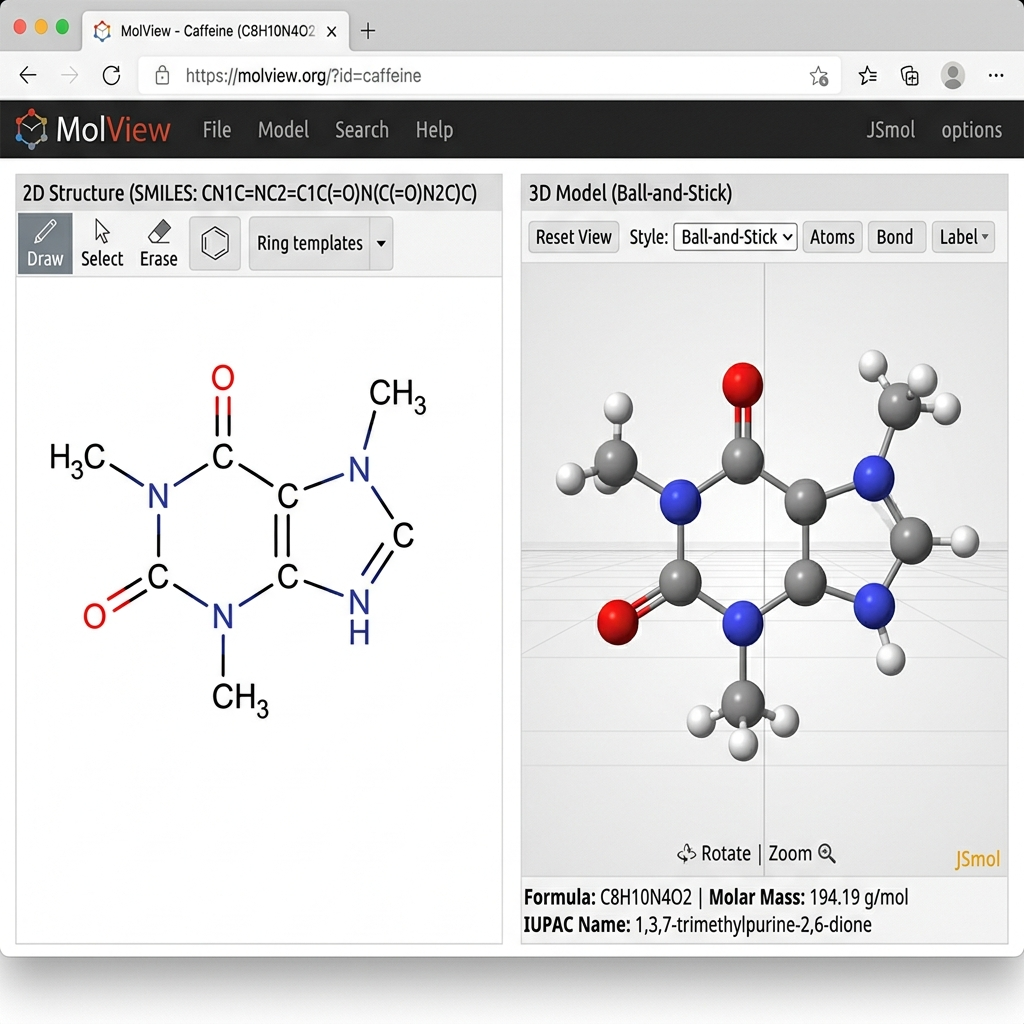
\includegraphics[width=0.72\linewidth]{images/molview_ui.jpg}
\caption[मॉलव्यू आणविक दृश्य अन्वेषण]{मॉलव्यू (MolView) वेबसाइट का इंटरफ़ेस -- जहाँ बाईं ओर 2D संरचना और दाईं ओर कैफीन (Caffeine) अणु का 3D model (Ball-and-Stick) दर्शाया गया है।}
\label{fig:molview-ui}
\end{figure}

% ---------------- परियोजना ----------------
\begin{pariyojana}[विलेयता का पूर्वानुमान - प्रयोग से सत्यापन]
\textbf{उद्देश्य:} वास्तविक प्रयोग का data एकत्र कर उससे पूर्वानुमान करना एवं उसे
प्रयोग से जाँचना।\\[4pt]
\textbf{सामग्री:} सामान्य नमक या चीनी, जल, बीकर, थर्मामीटर, तुला (balance)।\\[4pt]
\textbf{कार्य (समूह में, 3–4 विद्यार्थी):}
\begin{enumerate}[leftmargin=1.6em]
  \item विभिन्न तापमानों (जैसे 20, 30, 40, 50\,$^\circ$C) पर 100\,mL जल में अधिकतम
        घुलने वाले पदार्थ की मात्रा मापें।
  \item ताप बनाम विलेयता का ग्राफ़ बनाएँ तथा सर्वोत्तम रेखा/वक्र खींचें।
  \item ग्राफ़ से किसी \emph{नए} तापमान (जैसे 35\,$^\circ$C) पर विलेयता का पूर्वानुमान करें।
  \item अब वास्तव में उस ताप पर मापकर पूर्वानुमान की त्रुटि ज्ञात करें।
  \item चर्चा करें - data बिंदु बढ़ाने पर पूर्वानुमान बेहतर हुआ या नहीं?
\end{enumerate}
\textbf{मूल्यांकन:} मापन की शुद्धता, ग्राफ़, पूर्वानुमान-त्रुटि एवं निष्कर्ष की
स्पष्टता के आधार पर।
\end{pariyojana}

% ---------------- सारांश ----------------
\section*{सारांश (Summary)}
\addcontentsline{toc}{section}{सारांश}
\begin{itemize}[leftmargin=1.4em]
  \item अणु को संरचना/SMILES के रूप में संख्याओं में बदलकर AI लाखों अणुओं की तुलना
        कर सकती है।
  \item आवर्त सारणी की प्रवृत्तियाँ पैटर्न-पहचान एवं पूर्वानुमान का उत्कृष्ट उदाहरण हैं।
  \item रसायन में AI के दो प्रमुख कार्य हैं - वर्गीकरण (classification) एवं
        गुण-पूर्वानुमान (prediction)।
  \item दवा-खोज, नई सामग्री एवं हरित रसायन में AI समय एवं लागत बहुत घटा देती है।
  \item मुफ़्त उपकरण (MolView, PubChem) एवं सरल Python से विद्यार्थी स्वयं यह अनुभव कर
        सकते हैं।
\end{itemize}

% ---------------- अभ्यास ----------------
\section*{अभ्यास (Exercises)}
\addcontentsline{toc}{section}{अभ्यास}
\textbf{अ. रिक्त स्थान भरिए:}
\begin{enumerate}[leftmargin=1.6em]
  \item अणु को एक पंक्ति (string) के रूप में लिखने की विधि \rule{2.8cm}{0.4pt} कहलाती है।
  \item किसी पदार्थ को ``अम्ल या क्षार'' श्रेणियों में बाँटना AI का \rule{2.8cm}{0.4pt} कार्य है।
  \item दवा-खोज में लाखों अणुओं को कंप्यूटर पर जाँचने को \rule{2.8cm}{0.4pt} कहते हैं।
\end{enumerate}

\textbf{ब. लघु उत्तरीय:}
\begin{enumerate}[leftmargin=1.6em]
  \item मेंडेलीफ़ का अनदेखे तत्वों का पूर्वानुमान आधुनिक ML से किस प्रकार मिलता है?
  \item classification एवं prediction (regression) में अंतर एक-एक रासायनिक उदाहरण से बताइए।
  \item दवा-खोज में AI के कोई तीन उपयोग लिखिए।
\end{enumerate}

\textbf{स. क्रियात्मक / दीर्घ उत्तरीय:}
\begin{enumerate}[leftmargin=1.6em]
  \item आवर्त-2 के तत्वों की त्रिज्या वाली गतिविधि कीजिए तथा अपने पूर्वानुमान की त्रुटि
        लिखिए।
  \item MolView पर तीन अणुओं की 3D संरचना देखिए और उनके SMILES संकेत लिखिए।
  \item ``AI नई दवाओं की खोज को कैसे तेज़ करती है'' - इस पर एक संक्षिप्त निबंध लिखिए।
\end{enumerate}

\begin{mcq}
  \item अणु को एक छोटी पंक्ति (string) के रूप में लिखने का संकेतन है:
    \begin{choices}\item SMILES \item HTML \item JSON \item SQL\end{choices}
  \item आवर्त सारणी में अनदेखे तत्वों का पूर्वानुमान किसने किया?
    \begin{choices}\item डाल्टन \item मेंडेलीफ़ \item रदरफोर्ड \item बोर\end{choices}
  \item कंप्यूटर पर लाखों अणुओं को जाँचकर दवा छाँटना कहलाता है:
    \begin{choices}\item आभासी छँटाई (virtual screening) \item आसवन
      \item क्रिस्टलन \item अनुमापन\end{choices}
  \item AI से खोजा गया नया एंटीबायोटिक (2020) था:
    \begin{choices}\item पेनिसिलिन \item हैलिसिन (Halicin)
      \item एस्पिरिन \item इंसुलिन\end{choices}
\end{mcq}

\begin{mukhyashabd}
\textbf{स्माइल्स संकेतन (SMILES)}, \textbf{वर्गीकरण (classification)},
\textbf{पूर्वानुमान (prediction)}, \textbf{आभासी छँटाई (Virtual Screening)},
\textbf{गुण-पूर्वानुमान (Property Prediction)}, \textbf{अणु-अभिकल्प (Molecule Design)},
\textbf{उत्प्रेरक (catalyst)}।
\end{mukhyashabd}
\selfcheckqr{https://kkreboot.github.io/ai-in-science-hindi/quiz/ch3.html}
